\section{Python execution functions}

\subsection{xlpSet}

\begin{xlpfunctitle}{xlpSet}

\begin{xlpfunc}{Parameters}
\begin{tabular}{p{3.5cm}cl}
\textbf{scalar}& : & scalar code \\
\textbf{args}& : & list or arguments \\
\textbf{values}& : & list of values \\
\textbf{index}& : & list of index  \\
\textbf{id}& : & object id \\
\textbf{trigger}& : & trigger \\
\end{tabular}

\vspace{2mm}

index and values must have the same size if index is passed.
\end{xlpfunc}


\begin{xlpfunc}{Returns}
A character string representing the python object created
\end{xlpfunc}

\begin{xlpfunc}{Description}
Execute python code and store the result into a python object. It is the core function of \xlp. 

\

The values and index argument are used to fill container in a generic way.

\

The function creates an object with the scalar and args information. If the argument values is not empty and the object implement the \_\_setitem\_\_ method, the function will try to fill the object with the data contained in values. 

If the index argument is not empty, the elements of index argument will be used as the index parameter of the \_\_setitem\_\_ method. Otherwise, $\{1, ..., n\}$ will be used.

\

\textbf{Argument bindings} : \_args, \_size, \_rows, \_cols, \_1 ... \_n

\

If the scalar argument corresponds to a python code that does not return an object, xlpSet will return an object of NoneType. 

\

values and index arguments are automatically reduce (see xlpReduce for more details).

\

Two local function are available for creating objects:
\begin{itemize}
\item \_listlist(rows, columns, args): that create a list of list of dimenstions (rows, columns) filling the data with arguments (cf. xlp-example.xls).
\item \_extstr(rows, columns, args): that create a string from a cell matrix putting tabular character when a column jump appears and new line character when a row jump appears (cf. xlp-example.xls).
\end{itemize}

\end{xlpfunc}

\end{xlpfunctitle}

\subsection{xlpGet}

\begin{xlpfunctitle}{xlpGet}

\begin{xlpfunc}{Parameters}
\begin{tabular}{p{3.5cm}cl}
\textbf{scalar}& : & scalar code \\
\textbf{args}& : & list or arguments \\
\textbf{transpose}& : & transpose   \\
\textbf{trigger}& : & trigger \\
\end{tabular}

\vspace{2mm}

\end{xlpfunc}


\begin{xlpfunc}{Returns}
A cell matrix.
\end{xlpfunc}

\begin{xlpfunc}{Description}
Get data from python and display it in Excel. This method is generic and can handled only types:
\begin{itemize}
\item float
\item str
\item bool
\item NoneType
\item complex
\item other types that implement {\sl \_\_getitem\_\_} method and/or the {\sl size} method. 
\end{itemize}

The {\sl size} method return a tuple with the dimensions of the object to show. Obviously \xlp cannot handle more than two dimensions. That means that a matrix object will return a tuple of size 2 and a vector a tuple of size 1.

\

xlpGet as a specific behaviour with character string. \xlp interprets the tabular caharacter to jump to a new column and the new line character to jump to a new row. That means that this sentence "Hello <tabular> this	<tabular> is a <newline> test <tabular>	message	<newline> The name <tabular> of <tabular>	XLPython <newline> is	<tabular> XLPython" will be show as: 

\

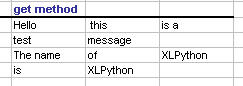
\includegraphics[width=6cm]{images/extstr2.jpg}


\

\textbf{Argument bindings} : \_args, \_size, \_rows, \_cols, \_1 ... \_n



\end{xlpfunc}
\end{xlpfunctitle}



\subsection{xlpPrettyGet}

\begin{xlpfunctitle}{xlpCommandGet}

\begin{xlpfunc}{Parameters}
\begin{tabular}{p{3.5cm}cl}
\textbf{scalar}& : & scalar code \\
\textbf{args}& : & list or arguments \\
\textbf{output}& : & output cell matrix\\
\textbf{transpose}& : & transpose   \\
\end{tabular}

\vspace{2mm}

\end{xlpfunc}


\begin{xlpfunc}{Returns}
A cell matrix.
\end{xlpfunc}

\begin{xlpfunc}{Description}
Same as xlpGet but the result is written on the ouput cell matrix. This function can only be called from VBA. "success" is returned in case of success or "more" if the output cell matris is not big enough to contain all the result.
\end{xlpfunc}
\end{xlpfunctitle}


\subsection{xlpApply}

\begin{xlpfunctitle}{xlpApply}

\begin{xlpfunc}{Parameters}
\begin{tabular}{p{3.5cm}cl}
\textbf{scalar}& : & scalar code \\
\textbf{args}& : & list or arguments \\
\textbf{id}& : & object id   \\
\textbf{trigger}& : & trigger \\
\end{tabular}

\vspace{2mm}

\end{xlpfunc}


\begin{xlpfunc}{Returns}
A character string representing the python object created
\end{xlpfunc}

\begin{xlpfunc}{Description}
Apply a callable object with args arguments.

\

\textbf{Argument bindings} : \_args, \_size, \_rows, \_cols, \_1 ... \_n

\end{xlpfunc}
\end{xlpfunctitle}


\subsection{xlpGetApply}

\begin{xlpfunctitle}{xlpGetApply}

\begin{xlpfunc}{Parameters}
\begin{tabular}{p{3.5cm}cl}
\textbf{scalar}& : & scalar code \\
\textbf{args}& : & list or arguments \\
\textbf{transpose}& : & transpose \\
\textbf{trigger}& : & trigger \\
\end{tabular}

\vspace{2mm}

\end{xlpfunc}


\begin{xlpfunc}{Returns}
A cell matrix.
\end{xlpfunc}

\begin{xlpfunc}{Description}
Apply a callable object with args arguments and return the result.

\

\textbf{Argument bindings} : \_args, \_size, \_rows, \_cols, \_1 ... \_n

\end{xlpfunc}
\end{xlpfunctitle}

\subsection{xlpCommandGetApply}

\begin{xlpfunctitle}{xlpPrettyGetApply}

\begin{xlpfunc}{Parameters}
\begin{tabular}{p{3.5cm}cl}
\textbf{scalar}& : & scalar code \\
\textbf{args}& : & list or arguments \\
\textbf{output}& : & output cell matrix\\
\textbf{transpose}& : & transpose
\end{tabular}

\vspace{2mm}

\end{xlpfunc}


\begin{xlpfunc}{Returns}
A cell matrix.
\end{xlpfunc}

\begin{xlpfunc}{Description}
The version of xlpCommandGet fo xlpGetApply.

\

\textbf{Argument bindings} : \_args, \_size, \_rows, \_cols, \_1 ... \_n

\end{xlpfunc}
\end{xlpfunctitle}












\subsection{xlpAttr}

\begin{xlpfunctitle}{xlpAttr}

\begin{xlpfunc}{Parameters}
\begin{tabular}{p{3.5cm}cl}
\textbf{scalar}& : & scalar code \\
\textbf{attr}& : & attribute \\
\textbf{args}& : & list or arguments \\
\textbf{id}& : & object id   \\
\textbf{trigger}& : & trigger \\
\end{tabular}

\vspace{2mm}

\end{xlpfunc}


\begin{xlpfunc}{Returns}
A character string representing the python object created
\end{xlpfunc}

\begin{xlpfunc}{Description}
Apply an attribute object with args arguments if callable or get an attribute object.

\

\textbf{Argument bindings} : \_args, \_size, \_rows, \_cols, \_1 ... \_n

\end{xlpfunc}
\end{xlpfunctitle}


\subsection{xlpGetAttr}

\begin{xlpfunctitle}{xlpGetAttr}

\begin{xlpfunc}{Parameters}
\begin{tabular}{p{3.5cm}cl}
\textbf{scalar}& : & scalar code \\
\textbf{args}& : & list or arguments \\
\textbf{transpose}& : & transpose \\
\textbf{trigger}& : & trigger \\
\end{tabular}

\vspace{2mm}

\end{xlpfunc}


\begin{xlpfunc}{Returns}
A cell matrix.
\end{xlpfunc}

\begin{xlpfunc}{Description}
Same as xlpAttr but returning directly the result and not an object.

\

\textbf{Argument bindings} : \_args, \_size, \_rows, \_cols, \_1 ... \_n

\end{xlpfunc}
\end{xlpfunctitle}

\subsection{xlpCommandGetAttr}

\begin{xlpfunctitle}{xlpPrettyGetAttr}

\begin{xlpfunc}{Parameters}
\begin{tabular}{p{3.5cm}cl}
\textbf{scalar}& : & scalar code \\
\textbf{args}& : & list or arguments \\
\textbf{output}& : & output cell matrix\\
\textbf{transpose}& : & transpose \\
\end{tabular}

\vspace{2mm}

\end{xlpfunc}


\begin{xlpfunc}{Returns}
A cell matrix.
\end{xlpfunc}

\begin{xlpfunc}{Description}
The version of xlpCommandGet fo xlpGetAttr

\

\textbf{Argument bindings} : \_args, \_size, \_rows, \_cols, \_1 ... \_n

\end{xlpfunc}
\end{xlpfunctitle}









\subsection{xlpExec}


\begin{xlpfunctitle}{xlpExec}

\begin{xlpfunc}{Parameters}
\begin{tabular}{p{3.5cm}cl}
\textbf{code}& : & script code \\
\textbf{args}& : & list or arguments \\
\textbf{ids}& : & list of ids \\
\textbf{transpose}& : & output transpose \\
\textbf{trigger}& : & trigger \\
\end{tabular}
\end{xlpfunc}


\begin{xlpfunc}{Returns}
A cell matrix of dimension (1, n) where n is the number of created objects  
\end{xlpfunc}

\begin{xlpfunc}{Description}
Execute python script written directly into Excel cells. The returns cell matrix represent the object ids.


\

A special object is available in order to return data. This object is "\_" and has just one method "operator+=". The usage is "\_ += object\_to\_return" in order to allow object to be available in Excel.

If you define any object into your code, you can also declare it as global in order that it will be available for future python call.

\

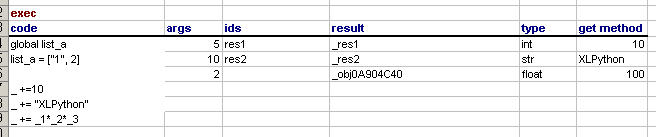
\includegraphics[width=11cm]{images/exec.jpg}

\

\textbf{Argument bindings} : \_args, \_size, \_rows, \_cols, \_1 ... \_n
 
\end{xlpfunc}
\end{xlpfunctitle}



\subsection{xlpExecFile}


\begin{xlpfunctitle}{xlpExecFile}

\begin{xlpfunc}{Parameters}
\begin{tabular}{p{3.5cm}cl}
\textbf{code}& : & script code \\
\textbf{args}& : & list or arguments \\
\textbf{ids}& : & list of ids \\
\textbf{transpose}& : & output transpose \\
\textbf{trigger}& : & trigger \\
\end{tabular}
\end{xlpfunc}


\begin{xlpfunc}{Returns}
A cell matrix of dimension (1, n) where n is the number of created object  
\end{xlpfunc}

\begin{xlpfunc}{Description}
Same as xlpExec but getting the python script from a file.

\

\textbf{Argument bindings} : \_args, \_size, \_rows, \_cols, \_1 ... \_n
 
\end{xlpfunc}
\end{xlpfunctitle}



\subsection{xlpImport}


\begin{xlpfunctitle}{xlpImport}

\begin{xlpfunc}{Parameters}
\begin{tabular}{p{3.5cm}cl}
\textbf{scalar}& : & scalar code\\
\textbf{id}& : & object id \\
\textbf{trigger}& : & trigger \\
\end{tabular}
\end{xlpfunc}


\begin{xlpfunc}{Returns}
A character string representing the object id of the imported module. 
\end{xlpfunc}

\begin{xlpfunc}{Description}
Import a python module with name given by id. If id is missing, the imported module name will be the same as the module name. 
\end{xlpfunc}
\end{xlpfunctitle}


\subsection{xlpFromImport}


\begin{xlpfunctitle}{xlpFromImport}

\begin{xlpfunc}{Parameters}
\begin{tabular}{p{3.5cm}cl}
\textbf{scalar}& : & scalar code\\
\textbf{trigger}& : & trigger \\
\end{tabular}
\end{xlpfunc}


\begin{xlpfunc}{Returns}
"success" in case of no error. 
\end{xlpfunc}

\begin{xlpfunc}{Description}
Same as "from module\_name" import *. 
\end{xlpfunc}
\end{xlpfunctitle}


\subsection{xlpFromImport}


\begin{xlpfunctitle}{xlpInsertPaths}

\begin{xlpfunc}{Parameters}
\begin{tabular}{p{3.5cm}cl}
\textbf{paths}& : & list of paths to include \\
\textbf{trigger}& : & trigger \\
\end{tabular}
\end{xlpfunc}


\begin{xlpfunc}{Returns}
"success" in case of no error.
\end{xlpfunc}

\begin{xlpfunc}{Description}
Insert paths in the python system path (check for duplication).
\end{xlpfunc}
\end{xlpfunctitle}


